\begin{figure}
%	\setlength\abovecaptionskip{0.5\baselineskip}
%  	\setlength\abovecaptionskip{0.75\baselineskip}
        \begin{center}
    		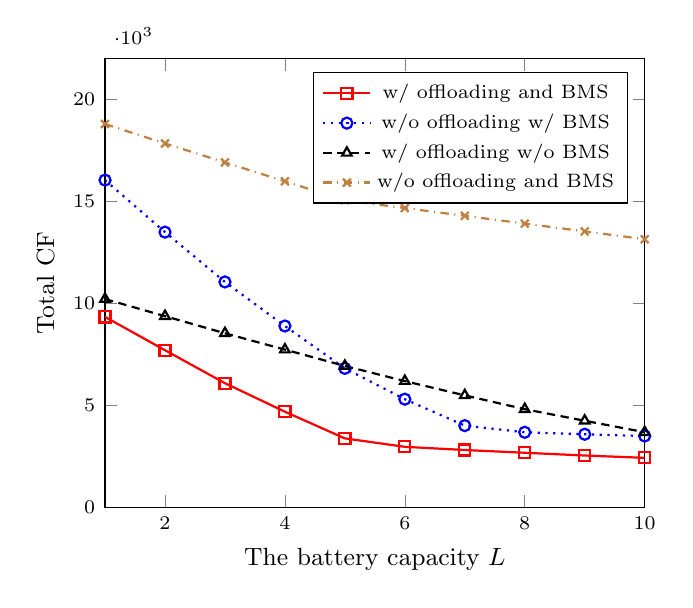
\begin{tikzpicture}
        		\begin{axis}[
        		%	scaled ticks=true, 
        		%	scaled y ticks={real:1e3},
        			scaled y ticks=base 10:-3,
        		    %title={},
        		    xlabel={The battery capacity $L$},
        		    ylabel={Total CF},
        		    xmin=1, xmax=10,
        		    ymin=0, ymax=22000,
        		  %  xtick={25, 50, 75, 100, 125, 150},
        		%	xticklabels=\empty,
        %		    ytick={0, 1000, 2000, 3000},
        		%	point meta=y *10^3, % the displayed number
        		    legend pos=north east,
        		    %ymajorgrids=true,    
        		    %xmajorgrids=true,
        		    grid style=densely dashed,
        		    tick label style={font=\scriptsize},
        		    label style={font=\small},
        		    legend style={font=\scriptsize},
        		]
        		
            		\addplot[ color=red, mark=square, line width=0.8pt]     
            		coordinates { 
            		( 1 , 9342.1 )
                    ( 2 , 7706.7 )
                    ( 3 , 6087.9 )
                    ( 4 , 4689.1 )
                    ( 5 , 3379.7 )
                    ( 6 , 2966.0 )
                    ( 7 , 2809.3 )
                    ( 8 , 2674.2 )
                    ( 9 , 2539.1 )
                    ( 10 , 2425.4 )
            		};
            		%
            		\addplot[ color=blue, mark=o, dotted, mark options={solid}, line width=0.8pt]     
            		coordinates {
                    ( 1 , 16053.6 )
                    ( 2 , 13501.4 )
                    ( 3 , 11056.8 )
                    ( 4 , 8895.2 )
                    ( 5 , 6815.0 )
                    ( 6 , 5303.2 )
                    ( 7 , 4006.2 )
                    ( 8 , 3679.6 )
                    ( 9 , 3582.6 )
                    ( 10 , 3496.2 )
            		};
            		
            		\addplot[ color=black, mark=triangle, densely dashed, mark options={solid}, line width=0.8pt]
            		coordinates {
                    ( 1 , 10218.3 )
                    ( 2 , 9378.0 )
                    ( 3 , 8537.7 )
                    ( 4 , 7735.5 )
                    ( 5 , 6933.3 )
                    ( 6 , 6190.4 )
                    ( 7 , 5490.7 )
                    ( 8 , 4812.6 )
                    ( 9 , 4245.1 )
                    ( 10 , 3682.4 )
            		};
            		
            		\addplot[ color=brown, mark=x, dash dot, mark options={solid}, line width=0.8pt]
            		coordinates {
                    ( 1 , 18807.0 )
                    ( 2 , 17852.0 )
                    ( 3 , 16923.0 )
                    ( 4 , 15994.0 )
                    ( 5 , 15065.0 )
                    ( 6 , 14683.0 )
                    ( 7 , 14301.0 )
                    ( 8 , 13919.0 )
                    ( 9 , 13537.0 )
                    ( 10 , 13155.0 )
            		};

            		\legend{w/ offloading and BMS, w/o offloading w/ BMS , w/ offloading w/o BMS, w/o offloading and BMS}
        		
        		\end{axis}
    		\end{tikzpicture}
    		
        \end{center}
    \caption{Caption.}\label{fig:result3}
\end{figure}
